\section{Exercise 1}
\subsection*{1.1}
When performing correlation and convolution we look at each pixel in the image at turn. The 'x' filter in this exercise looks at the pixel to the right and weights it by $1/2$, it looks at the pixel to the left and weights it $-1/2$, but the center pixel is not apparent in the formula, and is thus weighted zero. The same goes for the 'y' filter of the exercise. Thus we have:\\ 
'x' filter for convolution:	\begin{tabular}{|l|l|l|}
	\hline
	1/2 & 0 & -1/2 \\ \hline
\end{tabular}\\
'x' filter for correlation: \begin{tabular}{|l|l|l|}
	\hline
	-1/2 & 0 & 1/2 \\ \hline
\end{tabular}\\
'y' filter for convolution: \begin{tabular}{|l|}
		\hline
		1/2  \\ \hline
		0    \\ \hline
		-1/2 \\ \hline
	\end{tabular}\\
'y' filter for correlation: \begin{tabular}{|l|}
	\hline
	-1/2  \\ \hline
	0    \\ \hline
	1/2 \\ \hline
\end{tabular}\\
For all the filters the center pixel is the zero in the kernel. There is no difference between correlation and convolution if the kernel is symmetric. Given a Gaussian kernel is symmetric and a mean filter is constant (and thus also symmetric) there is no difference between convolution and correlation with these filters.

\subsection*{1.2}
Linearly separating the Sobel y derivative filter gives us:\\
\begin{equation*}
	f*\begin{bmatrix}
		1&2&1\\
		0&0&0\\
		-1&-2&-1
	\end{bmatrix}
 = f*\begin{bmatrix}
 	1\\
 	0\\
 	-1
 \end{bmatrix}
* \begin{bmatrix}
	1&2&1
\end{bmatrix}
\end{equation*}
Linearly separating the Prewitt y derivative filter gives us:\\
\begin{equation*}
	f*\begin{bmatrix}
		1&1&1\\
		0&0&0\\
		-1&-1&-1
	\end{bmatrix}
	= f*\begin{bmatrix}
		1\\
		0\\
		-1
	\end{bmatrix}
	* \begin{bmatrix}
		1&1&1
	\end{bmatrix}
\end{equation*}
We see that the separated y filter is almost identical to the one from the previous exercise, that is, we get almost the same result when convolving with the y filter alone. But for the Sobel and Prewitt filters we also convolve with an x filter afterwards, this means we involve more pixels in the convolution, and 'smooth' the noise more. We can look at the x filter as a 'smoothing' filter, as we are smoothing the image afterwards by adding the neighbouring pixel values to the center pixel. Because we involve more pixels in the convolution, the noisy pixels gets weighted less in total.

\subsection*{1.3}
\begin{figure}[H]
	\centering
	\begin{subfigure}[b]{\textwidth}
		\centering
		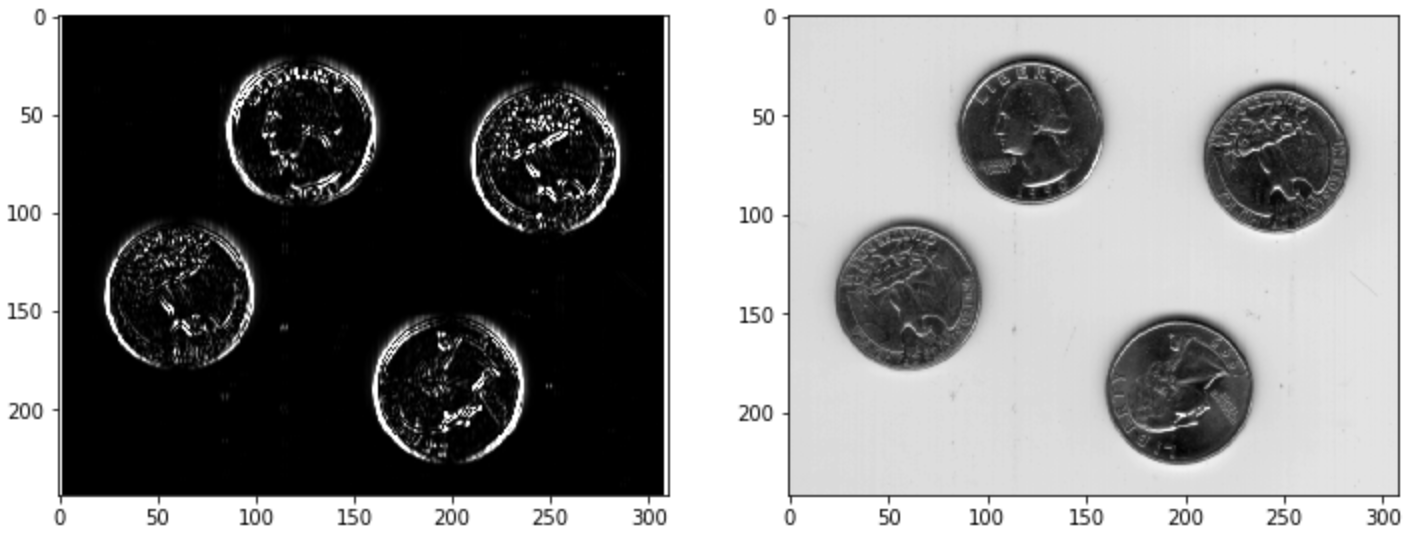
\includegraphics[width=\textwidth]{Materials/svar0}
		\caption{Variance 0}
	\end{subfigure}
	\hfill
	\\
	\begin{subfigure}[b]{\textwidth}
		\centering
		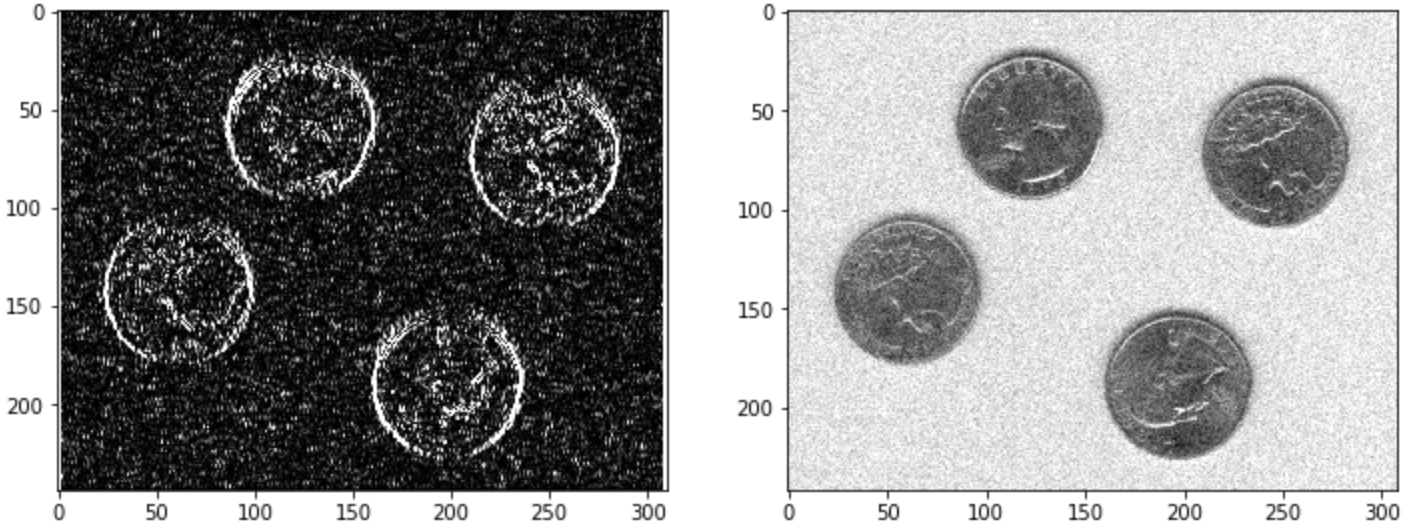
\includegraphics[width=\textwidth]{Materials/svar005}
		\caption{Variance 0.005}
	\end{subfigure}
	\hfill
	\\
	\begin{subfigure}[b]{\textwidth}
		\centering
		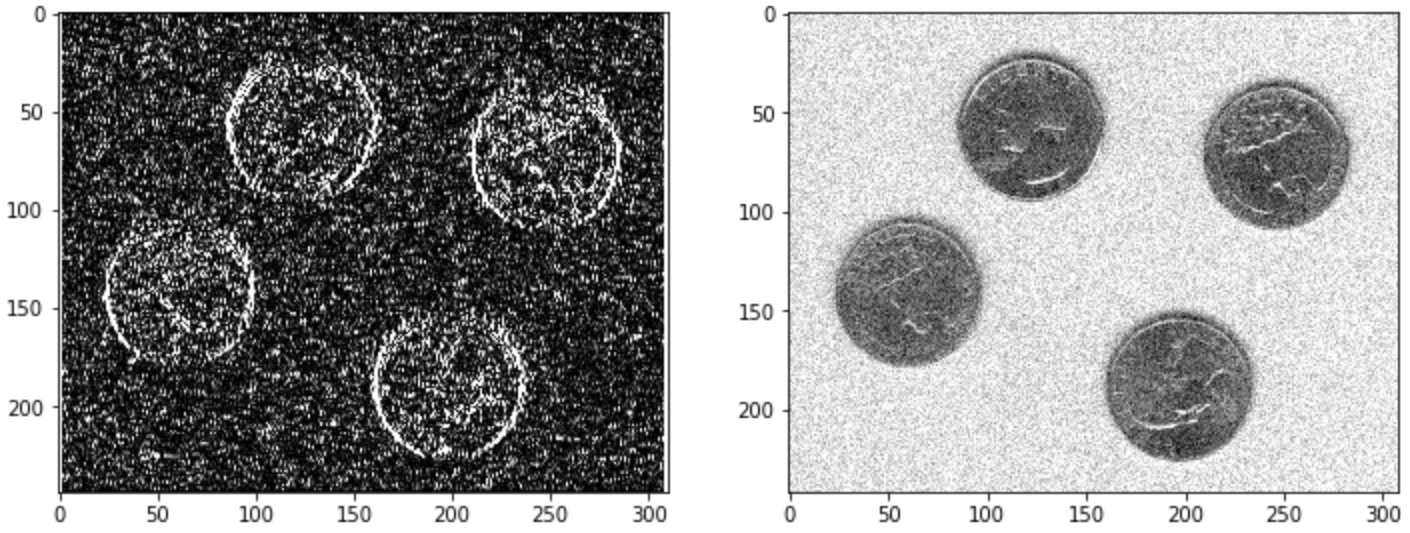
\includegraphics[width=\textwidth]{Materials/svar01}
		\caption{Variance 0.01}
	\end{subfigure}
	\caption{Gradients produced by filtering with Sobel.}
	\label{sobel1}
\end{figure}
\begin{figure}[H]
	\centering
	\begin{subfigure}[b]{0.85\textwidth}
		\centering
		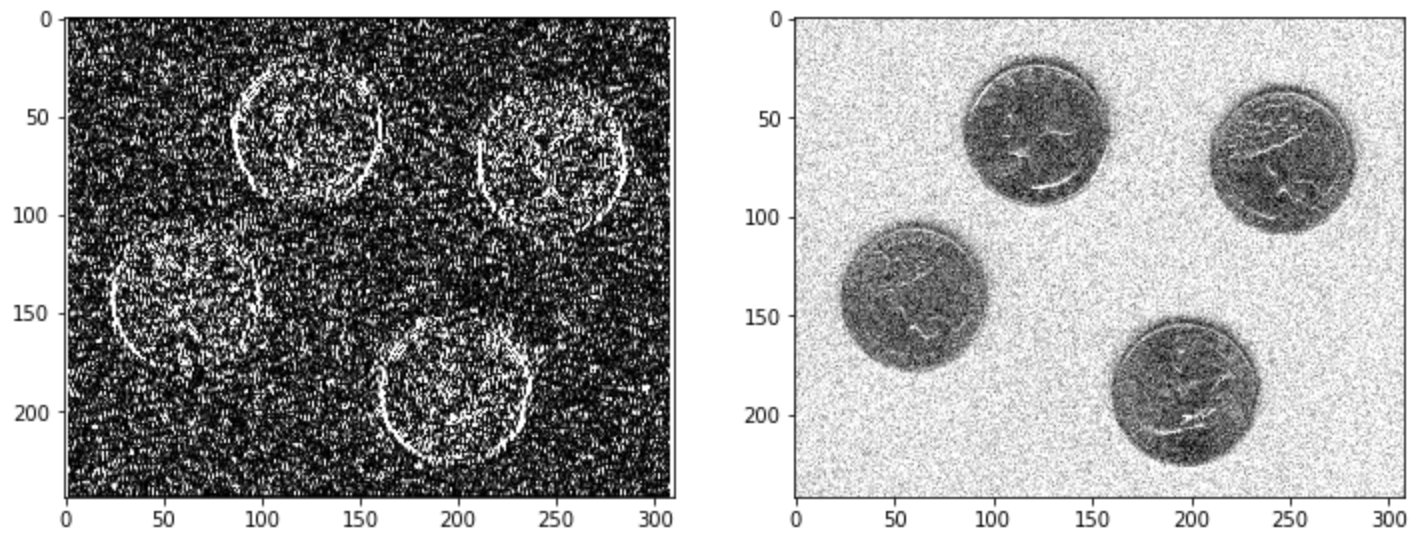
\includegraphics[width=\textwidth]{Materials/svar015}
		\caption{Variance 0.015}
	\end{subfigure}
	\hfill
	\\
	\begin{subfigure}[b]{\textwidth}
		\centering
		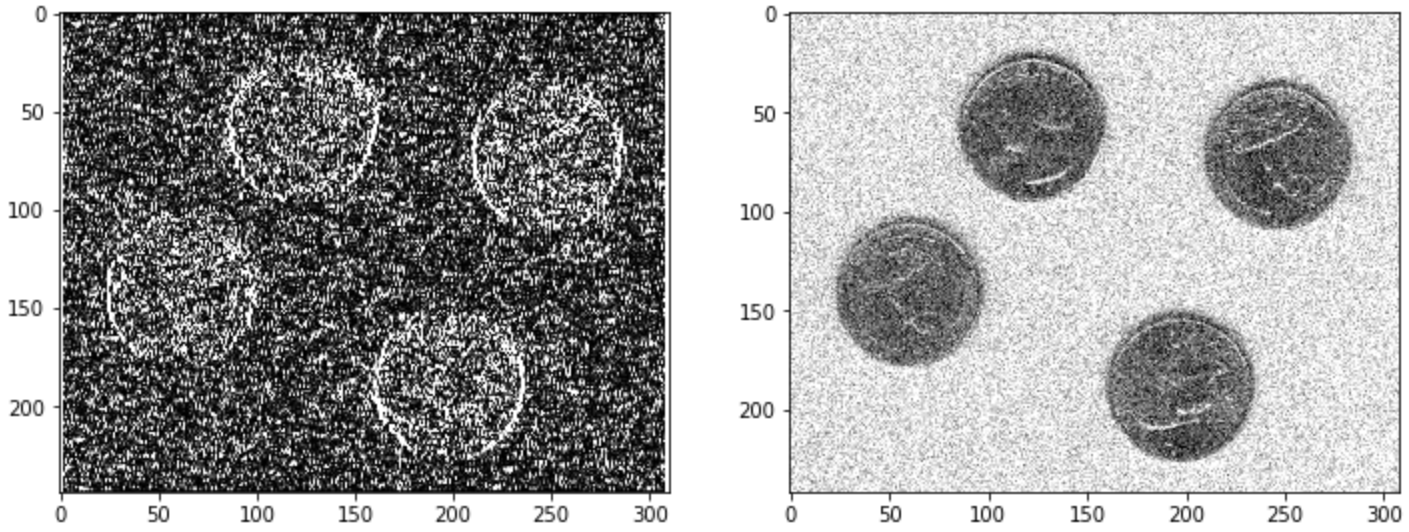
\includegraphics[width=0.85\textwidth]{Materials/svar02}
		\caption{Variance 0.02}
	\end{subfigure}
	\caption{Gradients produced by filtering with Sobel.}
	\label{sobel2}
\end{figure}

\begin{figure}[H]
	\centering
	\begin{subfigure}[b]{0.85\textwidth}
		\centering
		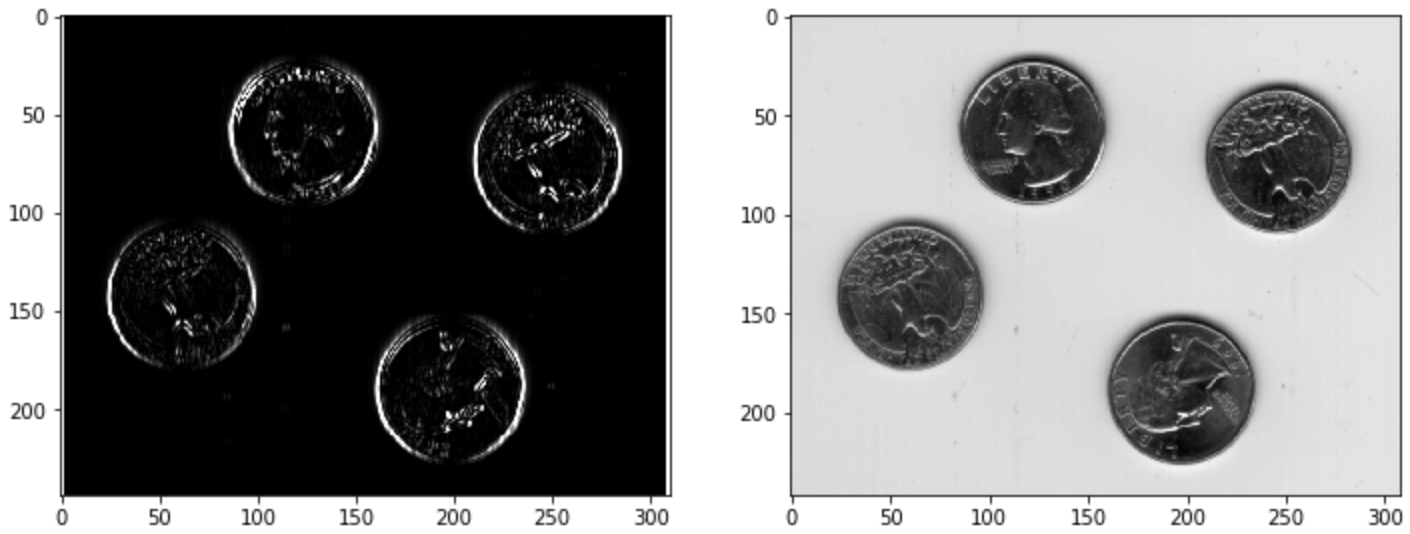
\includegraphics[width=\textwidth]{Materials/pvar0}
		\caption{Variance 0}
	\end{subfigure}
	\hfill
	\\
	\begin{subfigure}[b]{0.85\textwidth}
		\centering
		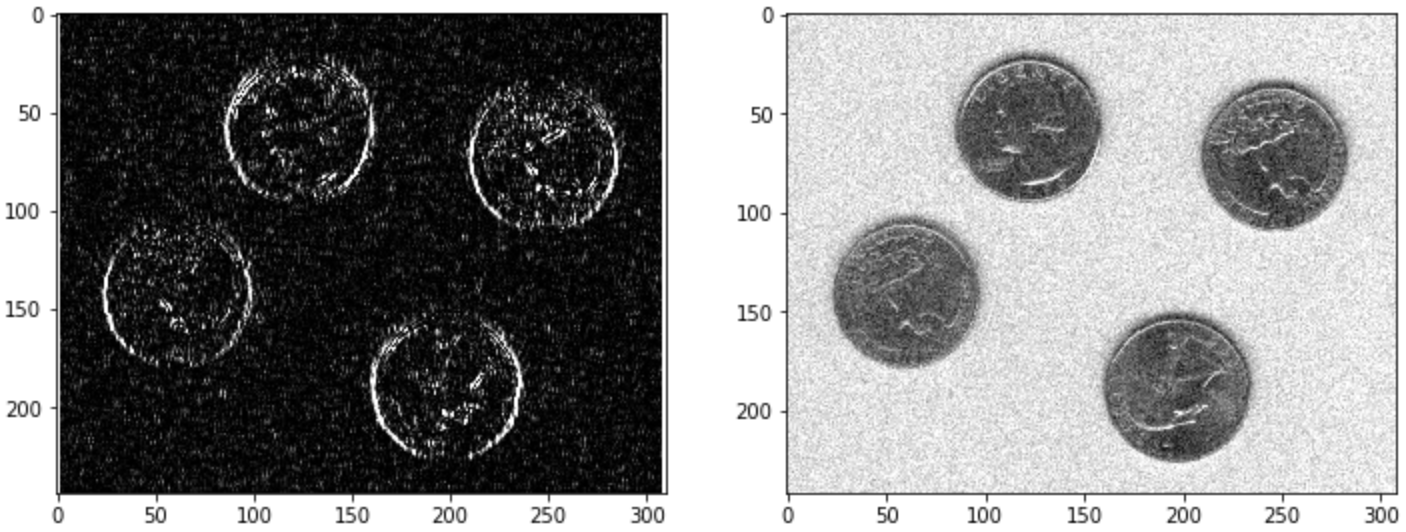
\includegraphics[width=\textwidth]{Materials/pvar005}
		\caption{Variance 0.005}
	\end{subfigure}
	\caption{Gradients produced by filtering with Prewitt.}
	\label{prewitt1}
\end{figure}
\begin{figure}[H]
	\centering
		\begin{subfigure}[b]{\textwidth}
		\centering
		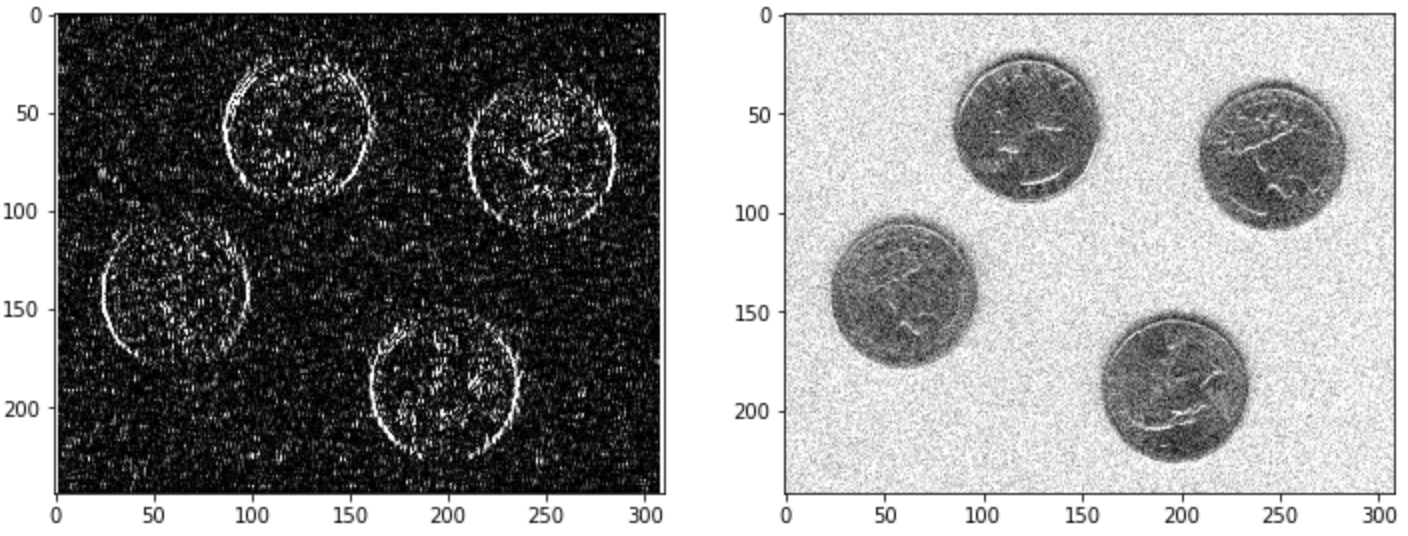
\includegraphics[width=\textwidth]{Materials/pvar01}
		\caption{Variance 0.01}
	\end{subfigure}
	\hfill
	\\
	\begin{subfigure}[b]{\textwidth}
		\centering
		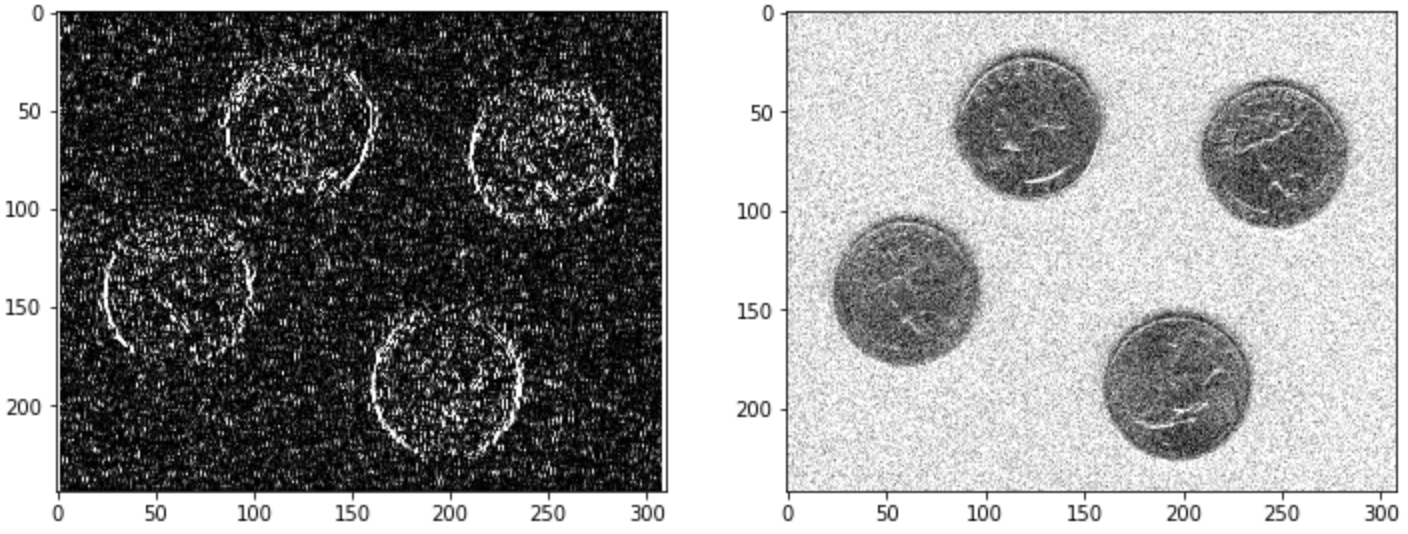
\includegraphics[width=\textwidth]{Materials/pvar015}
		\caption{Variance 0.015}
	\end{subfigure}
	\hfill
	\\
	\begin{subfigure}[b]{\textwidth}
		\centering
		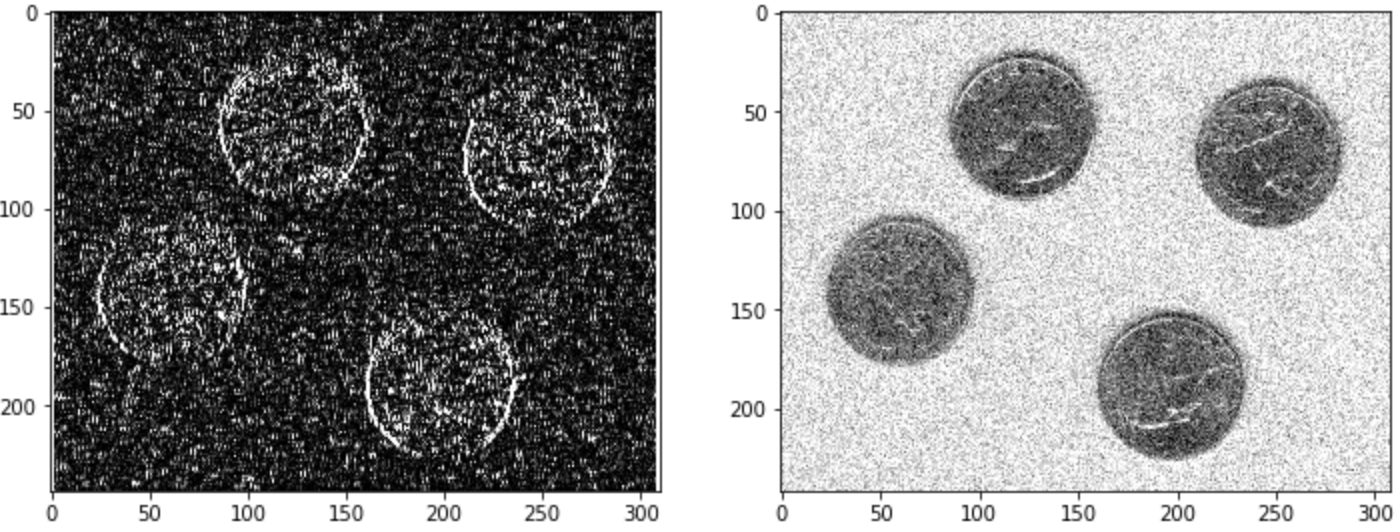
\includegraphics[width=\textwidth]{Materials/pvar02}
		\caption{Variance 0.02}
	\end{subfigure}
	\caption{Gradients produced by filtering with Prewitt.}
	\label{prewitt2}
\end{figure}
In \autoref{sobel1}, \autoref{sobel2}, \autoref{prewitt1} and \autoref{prewitt2} we see filtering with the Sobel and Prewitt filter for different variances. We see that the Prewitt filter seems to less effected by noise than the Sobel filter. Comparing the images with 0.2 variance it becomes somewhat hard to see the actual gradients with the Sobel filter whereas it is still rather clear in the Prewitt filter. However, the gradient is much more clear in the low variance images for the Sobel filter, where a lot more detail is also caught.\\
The code used for this exercise can be seen in \autoref{e1code}.
\begin{figure}[H]
	\centering
	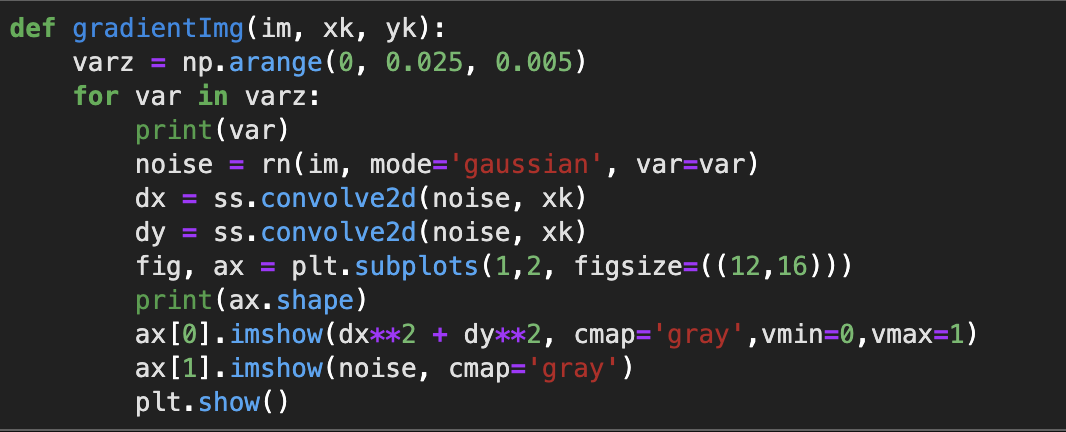
\includegraphics[width=0.7\linewidth]{Materials/e1code}
	\caption{Code for exercise 1.}
	\label{e1code}
\end{figure}